\documentclass[12pt]{article}

\usepackage{amsmath,amsthm,xspace,multirow}
\usepackage[margin=1in]{geometry}

\usepackage{amsmath} % essential for cases environment
\usepackage{amsthm} % for theorems and proofs
\usepackage{amsfonts} % mathbb
\usepackage{marvosym}
\usepackage{xspace}
\usepackage{multirow} % fancy tables
\usepackage{wasysym} % circle symbols (including half-filled circles)
\usepackage{enumerate} % fancier enumeration (e.g., a,b,c, ...)
%\usepackage{xcolor}
\usepackage{color}
\usepackage{mathtools}
\usepackage{tikz}
\usepackage{oubraces}
\usepackage{hyperref}
\usepackage[toc,page]{appendix}
\usepackage{cleveref}
\usepackage{cite}
\usepackage{textcomp}

\usepackage{algpseudocode,algorithm}
\usepackage{caption}
%used for spacing in list of figures/tables
\usepackage{tocloft}
%predominantly used for list of abbreviations and symbols
\usepackage{longtable}
\usepackage{enumitem}
	\newlist{abbrv}{itemize}{1}
	\setlist[abbrv,1]{label=,labelwidth=1in,align=parleft,itemsep=0.1\baselineskip,leftmargin=!}

%langauge
\usepackage[english]{babel}

%Tabular Commands
\usepackage{array}
\newcolumntype{L}[1]{>{\raggedright\let\newline\\\arraybackslash\hspace{0pt}}m{#1}}
\newcolumntype{C}[1]{>{\centering\let\newline\\\arraybackslash\hspace{0pt}}m{#1}}
\newcolumntype{R}[1]{>{\raggedleft\let\newline\\\arraybackslash\hspace{0pt}}m{#1}}

%make align work with lineno

\newcommand*\patchAmsMathEnvironmentForLineno[1]{%
  \expandafter\let\csname old#1\expandafter\endcsname\csname #1\endcsname
  \expandafter\let\csname oldend#1\expandafter\endcsname\csname end#1\endcsname
  \renewenvironment{#1}%
     {\linenomath\csname old#1\endcsname}%
     {\csname oldend#1\endcsname\endlinenomath}}% 
\newcommand*\patchBothAmsMathEnvironmentsForLineno[1]{%
  \patchAmsMathEnvironmentForLineno{#1}%
  \patchAmsMathEnvironmentForLineno{#1*}}%
\AtBeginDocument{%
\patchBothAmsMathEnvironmentsForLineno{equation}%
\patchBothAmsMathEnvironmentsForLineno{align}%
\patchBothAmsMathEnvironmentsForLineno{flalign}%
\patchBothAmsMathEnvironmentsForLineno{alignat}%
\patchBothAmsMathEnvironmentsForLineno{gather}%
\patchBothAmsMathEnvironmentsForLineno{multline}%
}

%commenting commands
\newcommand{\spenny}[1]{{\color{red}{(\bfseries Spenny: }{\em #1})}}
%\renewcommand{\spenny}[1]{}

%colours

\definecolor{dodgerblue}{RGB}{30,144,255}
\definecolor{darkorchid1}{RGB}{172,29,255}
\definecolor{orange}{RGB}{255,149,0}
\definecolor{forestgreen}{RGB}{0,122,16}
\newcommand{\red}[1]{{\color{red}#1}}

\newtheorem{theorem}{Theorem}[section]
\newtheorem{lemma}{Lemma}[section]
%\renewcommand\qedsymbol{\Coffeecup}
\newcommand{\Note}[1]{\textbf{\emph{Note:}\xspace#1}}
%Greek Letter shortcuts
\newcommand{\lam}{\lambda}
\newcommand{\Lam}{\Lambda}
\newcommand{\gam}{\gamma}
\newcommand{\Gam}{\Gamma}
\newcommand{\eps}{\varepsilon}


\newcommand{\ee}{(\hat{P_1},\hat{P_2},\hat{P_{12}})}
\newcommand{\eep}{\left(1-\frac{\mu}{f_1}\right)}
\newcommand{\eef}{\left(1-\frac{\mu}{f_1},0,0\right)}
\newcommand{\JD}[1]{{\color{blue}{\bfseries Jonathan:} #1}}
\newcommand{\EEZone}{\frac{\beta}{\alpha}\left(1-\frac{\mu}{\gam}\right)}

%Simulation Commands/Macros
\newcommand{\neigh}{{\cal N}}
\newcommand{\state}{\text{state}}
\newcommand{\cmax}[1]{\ensuremath c_{\rm #1}}
\newcommand{\heal}{\text{H}}
\newcommand{\susc}{\text{S}}
\newcommand{\expose}{\text{E}}
\newcommand{\infect}{\text{I}}


%Commenting commands:
\newcommand{\Question}[1]{{\em \bf Question:} #1}
\newcommand{\Answer}[1]{{\em \bf Answer:} #1}

%Unit commands
\newcommand{\mum}{\ensuremath \mu{\rm m}}
\newcommand{\cm}{\ensuremath {\rm cm}}
\newcommand{\mm}{\ensuremath {\rm mm}}

\newcommand{\f}{f}

%Equilibrium macros
\newcommand{\HE}{\textit{HE}\xspace}
\newcommand{\DE}{\textit{DE}\xspace}
\newcommand{\equil}{(\bar{H},\bar{S},\bar{E},\bar{I},\bar{V},\bar{Z})}
\newcommand{\eq}[1]{\overline{#1}}


%% macros
\newcommand{\Reals}{\mathbb{R}}
\newcommand{\term}[1]{{\bfseries\slshape #1}}
\newcommand{\Ker}{{\text{Ker}\,}}
\newcommand{\argmax}{{\text{argmax}}}
\newcommand{\argmin}{{\text{argmin}}}
\newcommand{\Range}{{\text{Range}\,}}
\newcommand{\norm}[1]{\left\|#1\right\|}
\newcommand{\abs}[1]{\left|#1\right|}
\newcommand{\R}{{\cal R}}
\newcommand{\G}{{\cal G}}
\newcommand{\N}{{\cal N}}
\newcommand{\Tinf}{T_\textrm{inf}}
\newcommand{\Prob}{\textrm{Pr}}
\newcommand{\Shat}{{\hat{S}}}
\newcommand{\Ihat}{{\hat{I}}}
\newcommand{\ie}{\emph{i.e., }}
\newcommand{\eg}{\emph{e.g., }}
% \newcommand{\Rlogo}{\protect\includegraphics[height=2ex,keepaspectratio]{images/Rlogo.pdf}\xspace}
\newcommand{\Rlogo}{\textbf{\textsf{R}}\xspace}
\newcommand{\XPPAUT}{\texttt{XPPAUT}\xspace}
\newcommand{\etal}{\textit{et al}.\xspace}
\newcommand\emphblue[1]{\emph{\color{blue}#1}}
\newcommand{\citehere}{{\large \bf CITE HERE}}

%derivative notation
\newcommand{\D}[2]{\frac{\mathrm{d}#1}{\mathrm{d}#2}}
\newcommand{\partD}[2]{\frac{\partial \mathrm{d}#1}{\partial #2 			\mathrm{d}t}}
\newcommand{\at}[2][]{\left. #1\right|_{#2}}
\newcommand{\partd}[2]{\frac{\partial #1}{\partial #2}}
\newcommand{\x}{\text{\bf x}}
\newcommand{\Mod}[1]{\ (\text{mod}\ #1)}
%THESE ARE SPENCER'S MACROSSSSSSS

\newcommand{\A}{\frac{\alpha\delta(\rho+\chi)}{\chi\beta f}}
\newcommand{\perday}{{$\text{day}^{-1}$\xspace}}

%Text Macros
\newcommand{\TM}{\textsuperscript{TM}\xspace}

\definecolor{dkgreen}{rgb}{0,0.6,0}
\definecolor{gray}{rgb}{0.5,0.5,0.5}
\definecolor{mauve}{rgb}{0.58,0,0.82}

%-----------------
% Listings Package for code script
%-----------------
\usepackage{listings}


\lstset{ %
  language=R,                     % the language of the code
  basicstyle=\footnotesize\ttfamily,       % the size of the fonts that are used for the code
  numbers=left,                   % where to put the line-numbers
  numberstyle=\tiny\color{gray},  % the style that is used for the line-numbers
  stepnumber=1,                   % the step between two line-numbers. If it's 1, each line
                                  % will be numbered
  numbersep=5pt,                  % how far the line-numbers are from the code
  backgroundcolor=\color{white},  % choose the background color. You must add \usepackage{color}
  showspaces=false,               % show spaces adding particular underscores
  showstringspaces=false,         % underline spaces within strings
  showtabs=false,                 % show tabs within strings adding particular underscores
  frame=none,                   % adds a frame around the code
  rulecolor=\color{black},        % if not set, the frame-color may be changed on line-breaks within not-black text (e.g. commens (green here))
  tabsize=2,                      % sets default tabsize to 2 spaces
  captionpos=b,                   % sets the caption-position to bottom
  breaklines=true,                % sets automatic line breaking
  breakatwhitespace=false,        % sets if automatic breaks should only happen at whitespace
  title=\lstname,                 % show the filename of files included with \lstinputlisting;
                                  % also try caption instead of title
  keywordstyle=\color{blue},      % keyword style
  commentstyle=\color{dkgreen},   % comment style
  stringstyle=\color{mauve},      % string literal style
  escapeinside={\%*}{*)},         % if you want to add a comment within your code
  morekeywords={*,...}            % if you want to add more keywords to the set
} 



\usepackage{tikz}
\usetikzlibrary{
arrows,decorations.pathmorphing,backgrounds,positioning,fit,calc,scopes,shapes.misc
}


\tikzset{
	auto,
	compartment/.style={
		rectangle, minimum size=9mm, rounded corners=2mm,
		thick, draw=black!15, top color=white,bottom color=black!30
	},
	%
	bigcompartment/.style={
		rectangle, minimum size=24mm, rounded corners=5mm,
		thick, draw=black!15, top color=white,bottom color=black!20
	},
	%
	point/.style={
		circle, inner sep=2pt, fill=black!5
	},
	%
	mytextbox/.style={
		rectangle, text=black!50, thin, 
		draw=white, top color=white,bottom color=white, fill=white
	}
	
}

\tikzset{cross/.style={cross out, draw=black, minimum size=2*(#1-\pgflinewidth), inner sep=0pt, outer sep=0pt},
%default radius will be 1pt. 
cross/.default={5pt}}

\newcommand{\SIRboxes}
{
\node (S) [bigcompartment,bottom color=blue!30]{{S}};
\node (SI) [right=of S]{};
\node (I) [bigcompartment,right=of SI,bottom color=red!30]{I};
\node (IR) [right=of I]{};
\node (R) [bigcompartment,right=of IR,bottom color=green!30]{R};
}
\newcommand{\sirvec}[2]{ 
	\draw[->, very thick] (S) to node[midway]{#1}(I) ;
	%\node (SIparam) [above of= SI]{#1}; 
	\draw[->, very thick] (I) to node[midway]{#2}(R);
	%\node (IRparam) [above of=IR]{#2}; 
}


\newcommand{\sirs}[1]{ 
	\draw[->, very thick] (R) 
		to  [bend left=45] node[midway] {#1} (S) ;
		 
}


\newcommand{\SIboxes}
{
\node (S) [bigcompartment,bottom color=blue!30]{{S}};
\node (SI) [right=of S]{};
\node (I) [bigcompartment,right=of SI,bottom color=red!30]{I};
}

\newcommand{\sivec}[1]{ 
	\draw[->, very thick] (S) to node[midway]{#1}(I) ;
	%\node (SIparam) [above of= SI]{#1};  
}

\newcommand{\sis}[1]
{
	\draw[->, very thick] (I) 
		to  [bend left=45] node[midway] {#1} (S) ;
}

\newcommand{\SILboxes}
{
\node (S) [bigcompartment,bottom color=blue!30]{S};
\node (SI) [right= of S]{};
\node (I) [bigcompartment,right=of SI,bottom color=red!30]{I};
\node (IL) [right=of I]{};
\node (L) [bigcompartment,right=of IL,bottom color=yellow!30]{L};
}







\usepackage{tikz}
\newdimen\mylw
\tikzset{chemeq/.style={draw,thick,double distance=2pt,onearc-onearc,/chemeq/size={#1}}}
\tikzset{chemeq/.default={.4pt 6pt}}
\pgfkeys{/chemeq/size/.code={\pgfsetarrowoptions{onearc}{#1}}}
\def\parseopts#1 #2{\xdef\myalw{#1}\xdef\myasize{#2}}
\pgfarrowsdeclare{onearc}{onearc}{%
  {\edef\x{\pgfgetarrowoptions{onearc}}\expandafter\parseopts\x}
  \mylw=\myalw
  \pgfarrowsleftextend{-\myasize-.5\mylw}
  \pgfarrowsrightextend{0pt}
}{%
  \pgfsetdash{}{0pt}
  {\edef\x{\pgfgetarrowoptions{onearc}}\expandafter\parseopts\x}
  \mylw=\pgflinewidth
  \pgfsetlinewidth{\myalw}
  \pgfpathmoveto{\pgfpoint{-\myasize}{-\myasize-.5\mylw}}%
  \pgfpatharc{180}{90}{\myasize}
  \pgfusepathqstroke
}

\title{Exploring the Effects of Vaccinating Men and Including Queer Interactions in HPV Transmission Models}
\author{Spencer Hunt and Dr. Jonathan Dushoff}
\begin{document}
\maketitle

\section{Introduction}
\begin{itemize}
\item brief HPV backgroun: virus that infects the epithelium; many different types spread sexually; associated with cervical cancer and other cancers.
\item Go into the history of vaccination: Gardasil and Cervarix, protected types, vaccination strategies in Canada (girls only)
\item Discuss some of the possible holes in this strategy: increased prevalence of oropharyngeal cancer in men with HPV, limited to no protection of queer men. 
\item Discuss some models previous results
\end{itemize}

\section{Methods}
\begin{itemize}
\item Introduce the model, flow and system of ODEs
\item Discuss the various types of sexual mixing models:
	\begin{enumerate}
	\item Separate men into heterosexual and queer, considers queer interactions
	\item Include queer men and heterosexual men into one group, still consider queer interactions 
	\item Only include men and women and heterosexual interactions
	\end{enumerate}	
\end{itemize}

\subsection{The Model}
We set up a mathematical model to illustrate the transmission of HPV.  Our model considers three different infection states: susceptible $S$, infected $I$, and vaccinated $V$.  Individuals are assigned to a state based on their infection status and move through the states due to transmission, vaccination, and recovery.  We consider a variety of different groups including men, women, queer men, and heterosexual men.  We illustrate the movement through the different classes as a flow diagram in figure~\ref{fig:flowDiag}.
\begin{figure}[h!]
\begin{center}
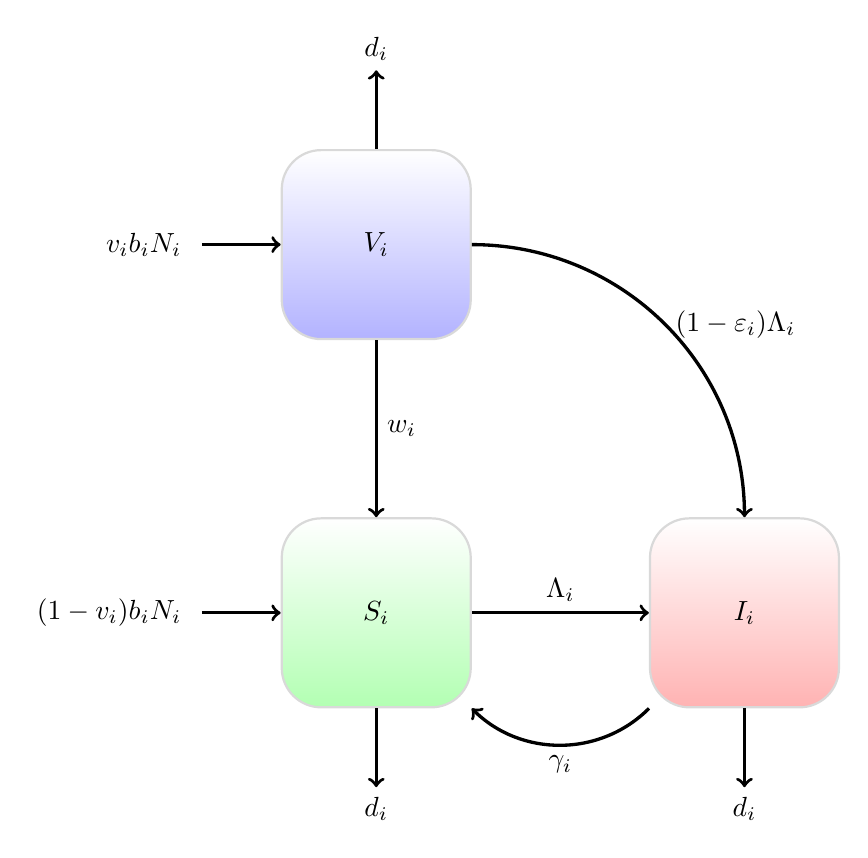
\begin{tikzpicture}
%compartments
\node (S)[bigcompartment, bottom color=green!30] {{$S_i$}};
\node (SI) [right =of S] {{}};
\node (I) [bigcompartment,right=of SI, bottom color=red!30] {{$I_i$}};
\node (SV) [above = of S] {{}};
\node (V) [bigcompartment,above=of SV, bottom color=blue!30] {{$V_i$}};

\node (leftS) [left=of S] {{}};
\node (leftV) [left=of V] {{}};
\node (downI) [below=of I] {{}};
\node (downS) [below=of S] {{}};
\node (upV) [above=of V] {{}};

%arrows
\draw[->,very thick] (S) to node[above] {$\Lambda_i$} (I);
\draw[->,very thick] (leftS) node[left] {$(1-v_i)b_iN_i$}  to (S);
\draw[->,very thick] (leftV) node[left] {$v_ib_iN_i$} to (V);
\draw[->,very thick] (V) to node[right] {$w_i$} (S);

\draw[->,very thick] (I) to[bend left=45] node[below] {$\gamma_i$} (S);
\draw[->, very thick] (V) to[bend left=45] node[right] {$(1-\eps_i)\Lambda_i$} (I);
\draw[->, very thick] (V) to (upV) node[yshift=1ex] {$d_i$};
\draw[->, very thick] (S) to (downS) node[yshift=-1ex] {$d_i$};
\draw[->, very thick] (I) to (downI) node[yshift=-1ex] {$d_i$};

\end{tikzpicture}
\caption{Flow diagram of the HPV transmsission model.}
\label{fig:flowDiag}
\end{center}
\end{figure}
The biological parameters $\Lambda_i$ and $\gamma_i$ represent the force of transmission for individuals and the recovery from HPV in group $i$, respectively.  We consider an SIS model here because natural infection with HPV does not prevent reinfection with the same type.  Vital parameters $b_i$ and $d_i$ represent the birth and death rates, respectively.  To simplify our model we consider a constant population and set $b_i=d_i$ for all groups $i$.  The population size of group $i$ is $N_i=S_i+I_i+V_i$.  We also consider various vaccination parameters.  The value of $v_i$ is the proportion of the population that is vaccinated entering the system.  The parameter $w_i$ represents the rate at which vaccination wanes.  Because the HPV vaccines are relatively new, it is not quite clear for how long they provide protection.  Therefore, $1/w_i$ is the average time that the vaccine provides protection.  Lastly, the parameter $\eps_i$ is the protective effects of the vaccine. This values ranges from 0 (no protection) to 1 (complete protection).  This model can also be represented as a system of differential equations below:
\begin{subequations}
\begin{align}
\dot{S_i} &= (1-v_i)b_iN_i + w_iV_i - \Lambda_iS_i + \gamma_i I_i - d_iS_i,\\
\dot{V_i} &= v_ib_iN_i - w_iV_i - (1-\eps_i)\Lambda_iV_i  - d_iV_i,\\
\dot{I_i} &=  \Lambda_i(S_i+(1-\eps_i)V_i) - \gamma_i I_i - d_iI_i.\end{align}
\end{subequations}


\subsection{Sexual Mixing}

In our paper, we set up three different scenarios for considering sexual mixing.

In the first scenario, we separate the men group into straight men $h$ and queer men $q$. The straight men have sex with women $w$ and queer men have sex with both other queer men and women.  We include queer women in the same group as straight women. Because vaccination strategies already target women, queer women benefit the greatest from the current vaccination strategies.  For this reason, we do not disentangle sexual interactions of queer women from straight women.  This scenario considers same-sex interactions and also actively tracts the infection of queer men.  

The second scenario still considers same-sex interactions, but queer men and straight men are contained within the same group, just referred to as men $m$.  

The last scenario only considers two groups, men and women, and only considers opposite-sex interactions.  Many HPV models up to this point only consider opposite-sex interactions, and this scenario in our paper is used to parallel the results to previous work.  Both groups of men and women here include queer and straight men and women, but we only consider opposite-sex interactions in the transmission of HPV. 
\section{Results}
\begin{itemize}
\item Discuss main results for each scenario of mixing and various vaccine coverage scenarios
\item Show pictures
\end{itemize}

\section{Next Steps}
\begin{itemize}
\item access data to estimate transmission parameters, fit to our model
\item perform a sensitivity analysis on  
\end{itemize}




\end{document}